\documentclass[10pt]{article}
\usepackage[margin=0.85in]{geometry}
\usepackage{booktabs}
\usepackage{microtype}
\usepackage{parskip}
\usepackage{titlesec}
\usepackage{hyperref}
\usepackage{graphicx}
\usepackage{caption}

\titleformat{\section}{\normalfont\bfseries\large}{\thesection}{0.6em}{}
\titlespacing*{\section}{0pt}{0.8em}{0.2em}
\captionsetup{font=small,labelfont=bf,skip=4pt}

\title{\vspace{-2.5em}\textbf{Decoder Alignment Is Not Feature Recovery in Sparse Autoencoders}\vspace{-0.5em}}
\author{}
\date{}

\begin{document}
\maketitle
\vspace{-3em}

\section*{The question, in one line}

When a sparse autoencoder (SAE) is trained on language model activations and one of its decoder vectors ends up pointing close to a meaningful direction in activation space, decoder geometry is often used as part of the evidence for interpreting that latent as a feature for that direction. But does geometric alignment actually mean the SAE has learned to use that direction as a clean, dedicated, selective unit? This artifact tests that question directly. At GPT-2-small scale, standard mixed-reconstruction SAEs can have nonzero decoder alignment with a target direction while failing to functionally recover it.

\section*{The setup}

Two ideas worth defining up front. \textbf{Decoder allocation} = how close, in cosine similarity, the SAE's best-matching decoder vector is to a target direction; this is the standard ``does the SAE point at this direction'' geometric measure. \textbf{Functional recovery} = whether the SAE actually produces a single latent that fires selectively when the target direction is present and reconstructs that component of the activation. These two come apart cleanly in what follows.

The experiments use controlled target directions injected into GPT-2-small residual-stream activations, across three direction groups: \textbf{weak} (low-SNR semantic directions), \textbf{strong} (high-SNR semantic directions), and \textbf{random} (random orthogonal directions). For each, SAEs are trained under four conditions:

\begin{enumerate}\setlength\itemsep{0em}\setlength{\parskip}{0pt}
  \item \textbf{L1 mixed}: standard SAE with L1 sparsity penalty, trained on mixed activations.
  \item \textbf{TopK mixed}: standard SAE with TopK sparsity, also on mixed activations.
  \item \textbf{Paired delta}: positive control. Trained on paired differences where the target direction is isolated. Intentionally easier than mixed training; its role is to show the directions are learnable in principle, not to argue paired-delta is a replacement for reconstruction SAEs.
  \item \textbf{Random-pair delta}: control for the positive control. Same delta structure but pairing is random, so no coherent target signal is isolated. Its failure rules out ``any pairwise training works.''
\end{enumerate}

Four quantities are logged at every training step: decoder allocation, target-gradient ratio, target residual explained, and best-latent selectivity. What the SAE has actually \emph{learned} (selectivity, recovery) is then compared against what its \emph{decoder geometry alone} suggests (allocation).

\section*{Paired-delta reaches near-perfect recovery; mixed reconstruction remains near chance}

The headline numbers at layer 8, scale 0.05, K=512 (averaged across the 10 target directions in each group):

\begin{center}\small
\begin{tabular}{lcccc}
\toprule
Group  & L1 mixed & TopK mixed & \textbf{Paired delta} & Random-pair \\
\midrule
weak   & 0.058 & 0.055 & \textbf{0.994} & 0.057 \\
strong & 0.063 & 0.059 & \textbf{0.994} & 0.052 \\
random & 0.057 & 0.054 & \textbf{0.994} & 0.057 \\
\bottomrule
\end{tabular}\\[0.2em]
{\footnotesize Mean recovery score (1.0 = perfect functional recovery, $\sim$0 = chance).}
\end{center}

Paired-delta reaches near-perfect recovery while mixed reconstruction stays near chance, producing roughly a 16$\times$ difference in mean recovery score, with random-pair flat at the same level as the two mixed conditions. The directions are learnable; the standard mixed objectives do not recover them as selective, functionally usable latents. The same pattern holds at K=2048, which reduces the possibility that the result is purely a capacity artifact; fully closing that objection would require K=4096--8192 (future work).

\begin{figure}[h]
\centering
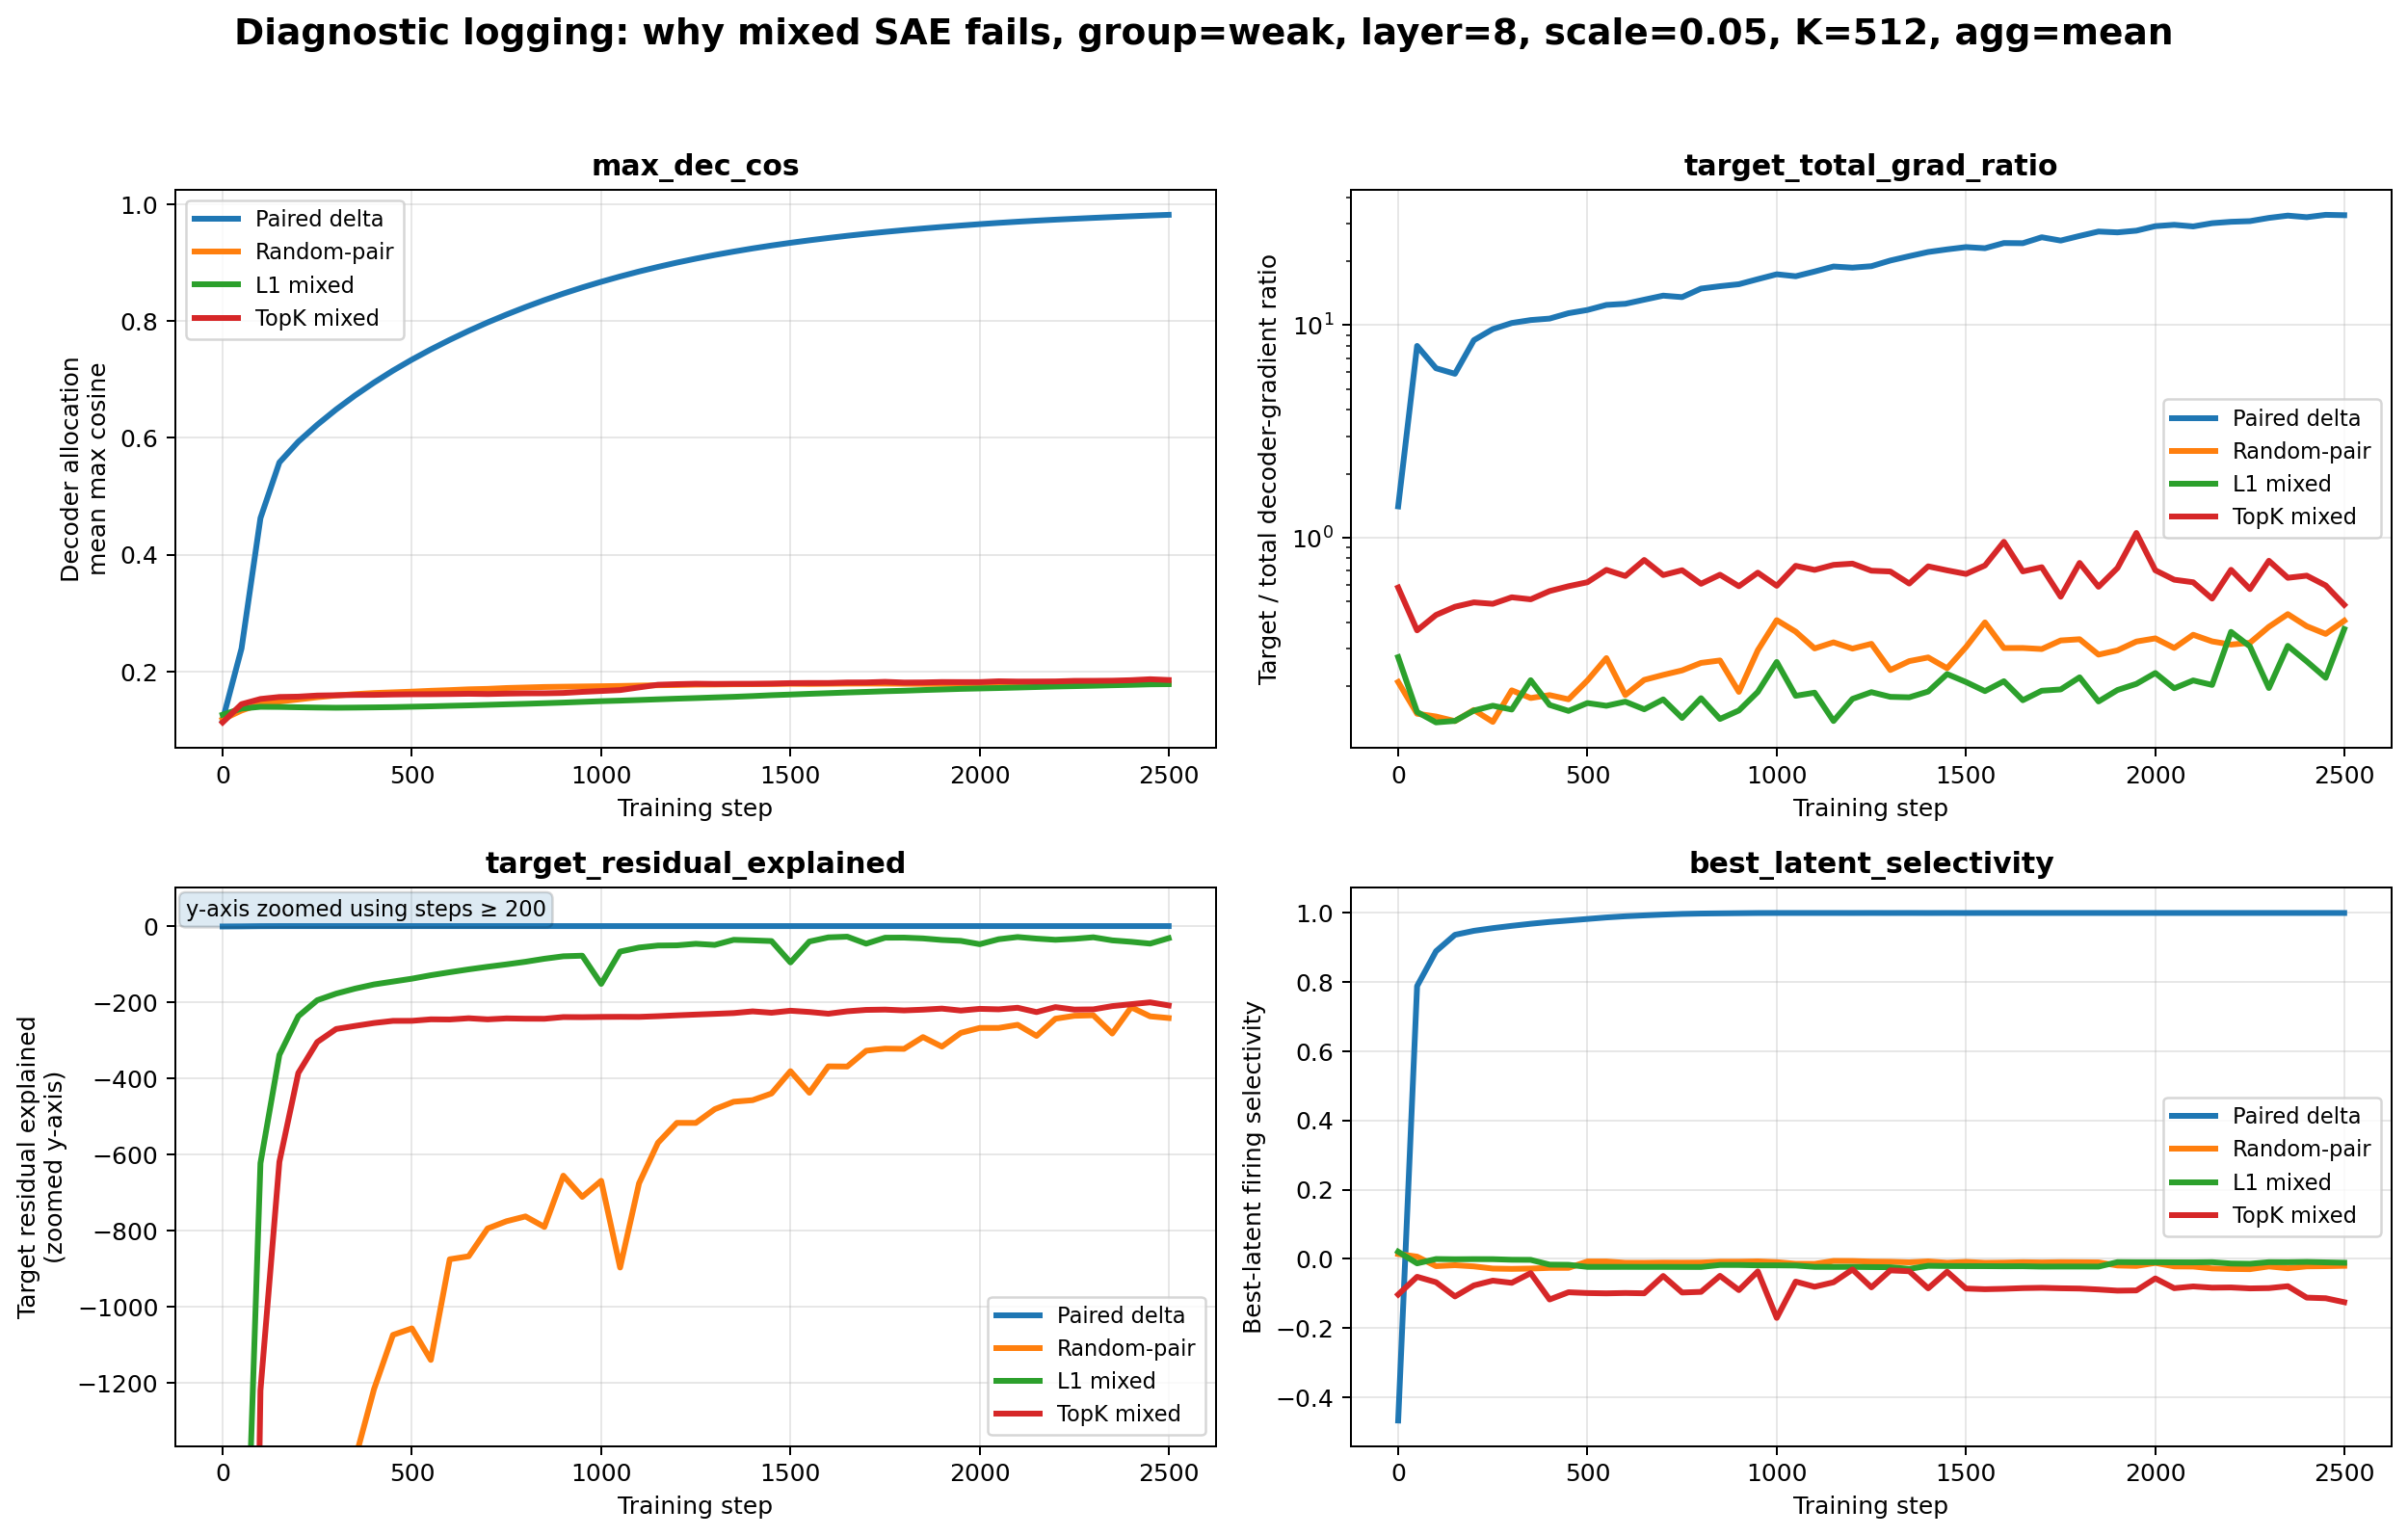
\includegraphics[width=0.75\linewidth]{figures/diagnostic_timeseries_weak_layer8_scale0.05_K512_zoom_agg.png}
\caption{Training dynamics for weak directions, averaged across 10 targets. Paired-delta climbs to $\sim$1 on decoder allocation, gets 30--60$\times$ more gradient pointed at the target, substantially improves the target-residual diagnostic, and produces a latent with $\sim$1.0 selectivity --- all within a few hundred steps. The other three conditions plateau on every metric and stay there for 2500 steps.}
\end{figure}

\section*{The failure isn't slow learning; it's structural}

The training curves rule out a simple alternative explanation. The mixed-SAE failure isn't ``the SAE is slowly working its way toward the target.'' The gradient pointed at the target sits at $\sim$0.3--1$\times$ the baseline rate (vs $\sim$30--60$\times$ for paired-delta), no single latent ever specialises to the target (selectivity stays near zero, sometimes slightly negative for TopK), and the target-residual diagnostic does not improve under mixed training. The picture is consistent with mixed training allocating capacity to other structure in the activations rather than forming a target-specific latent.

\section*{The conceptual point: alignment is not recovery}

Decoder allocation does \emph{not} stay at zero for mixed training. It sits at $\sim$0.18 (weak), $\sim$0.29 (strong), $\sim$0.12 (random) which is modestly above the noise floor, and large enough that a paper reporting ``the SAE has a decoder vector aligned with this direction'' would feel justified. But selectivity in those same SAEs is zero. Best-latent selectivity for TopK on strong targets is mildly \emph{negative}.

\begin{figure}[h]
\centering
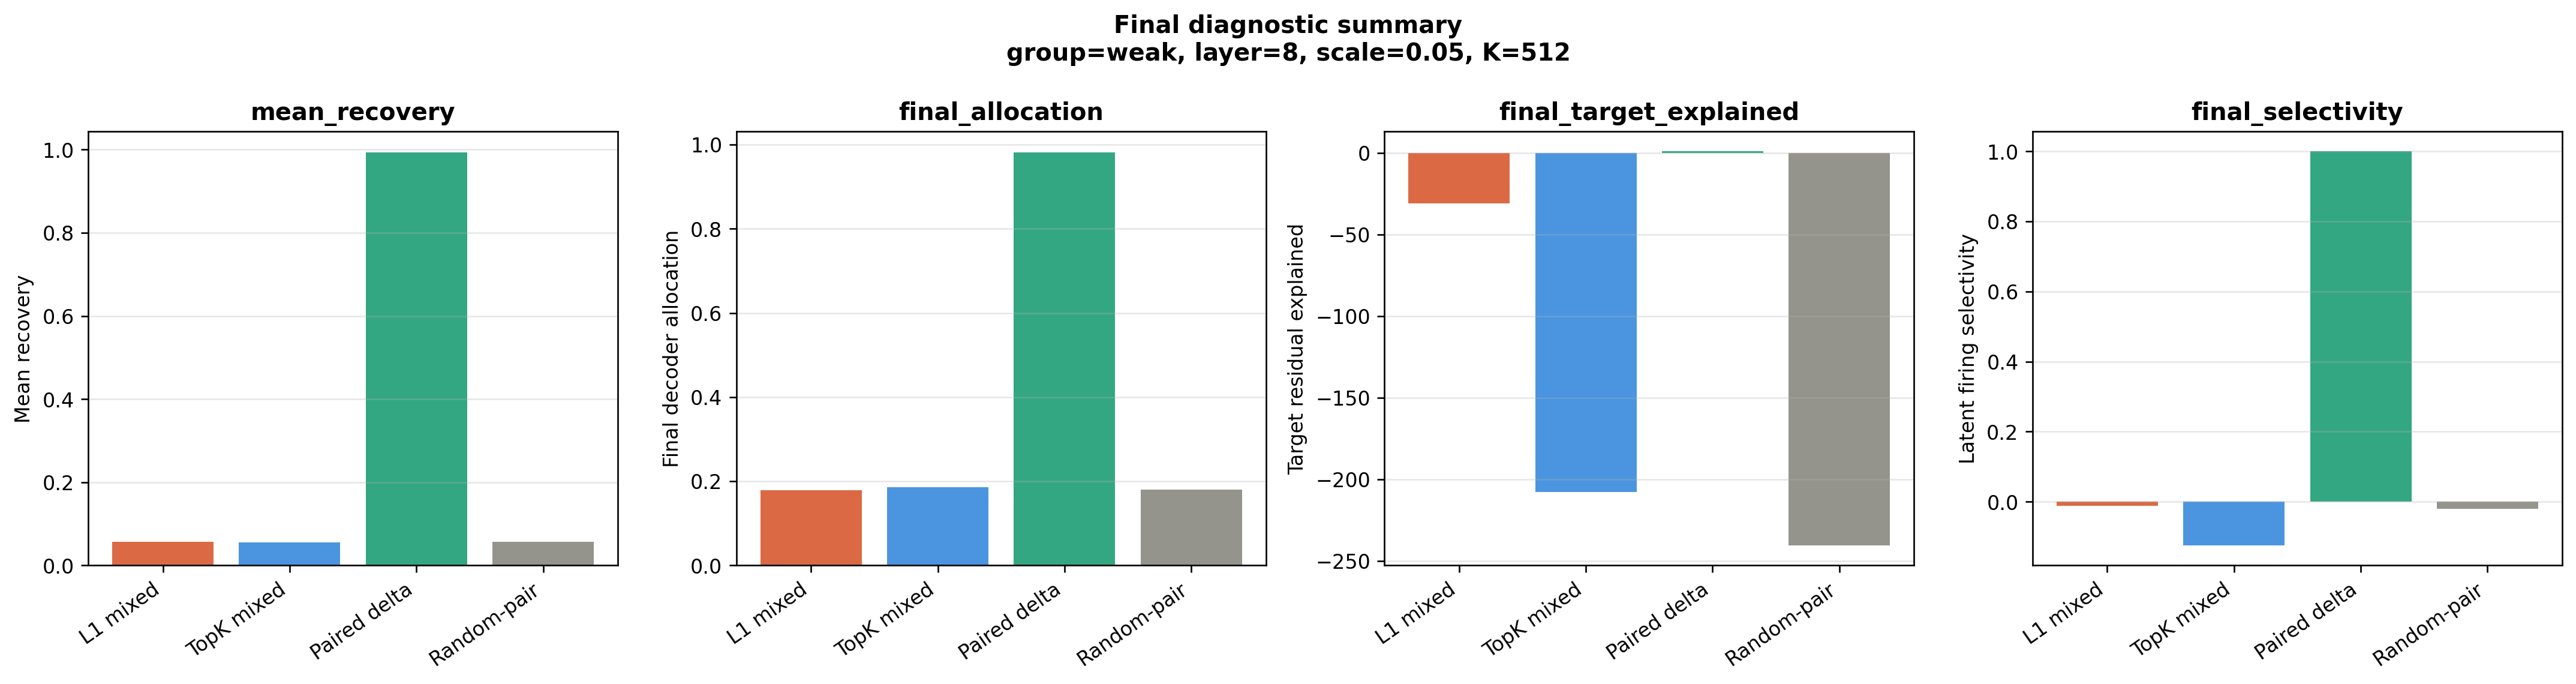
\includegraphics[width=0.75\linewidth]{figures/weak_diagnostic_final_bars_weak_layer8_scale0.05_K512.png}
\caption{Final state across the four metrics, weak group. Decoder allocation is meaningfully above zero for L1/TopK/random-pair (second panel). Recovery and selectivity are at chance (first and fourth panels). Geometric alignment without functional recovery.}
\end{figure}

So an SAE that appears to ``have a feature for'' a direction by the geometric criterion can still have no selective latent for that direction by the functional criterion. \textbf{Decoder alignment is not sufficient evidence of feature recovery.} The two diagnostics need to be reported together; either one on its own can mislead.

\section*{Public SAEs show comparable allocation levels}

To check this isn't a quirk of the internal training setup, the same allocation measurement was applied to a publicly released GPT-2-small residual-stream SAE. Public SAE allocation against the target directions sits at $\sim$0.28 (weak) and $\sim$0.36 (strong) which is roughly the same magnitude as the internal mixed SAEs, and well below the 0.95+ that paired-delta achieves. By an allocation-only diagnostic, the public SAE shows geometric evidence consistent with these directions. The paired-delta benchmark shows what alignment level the directions are actually capable of supporting, and the gap from that to what public training produces is large.

\begin{figure}[h]
\centering
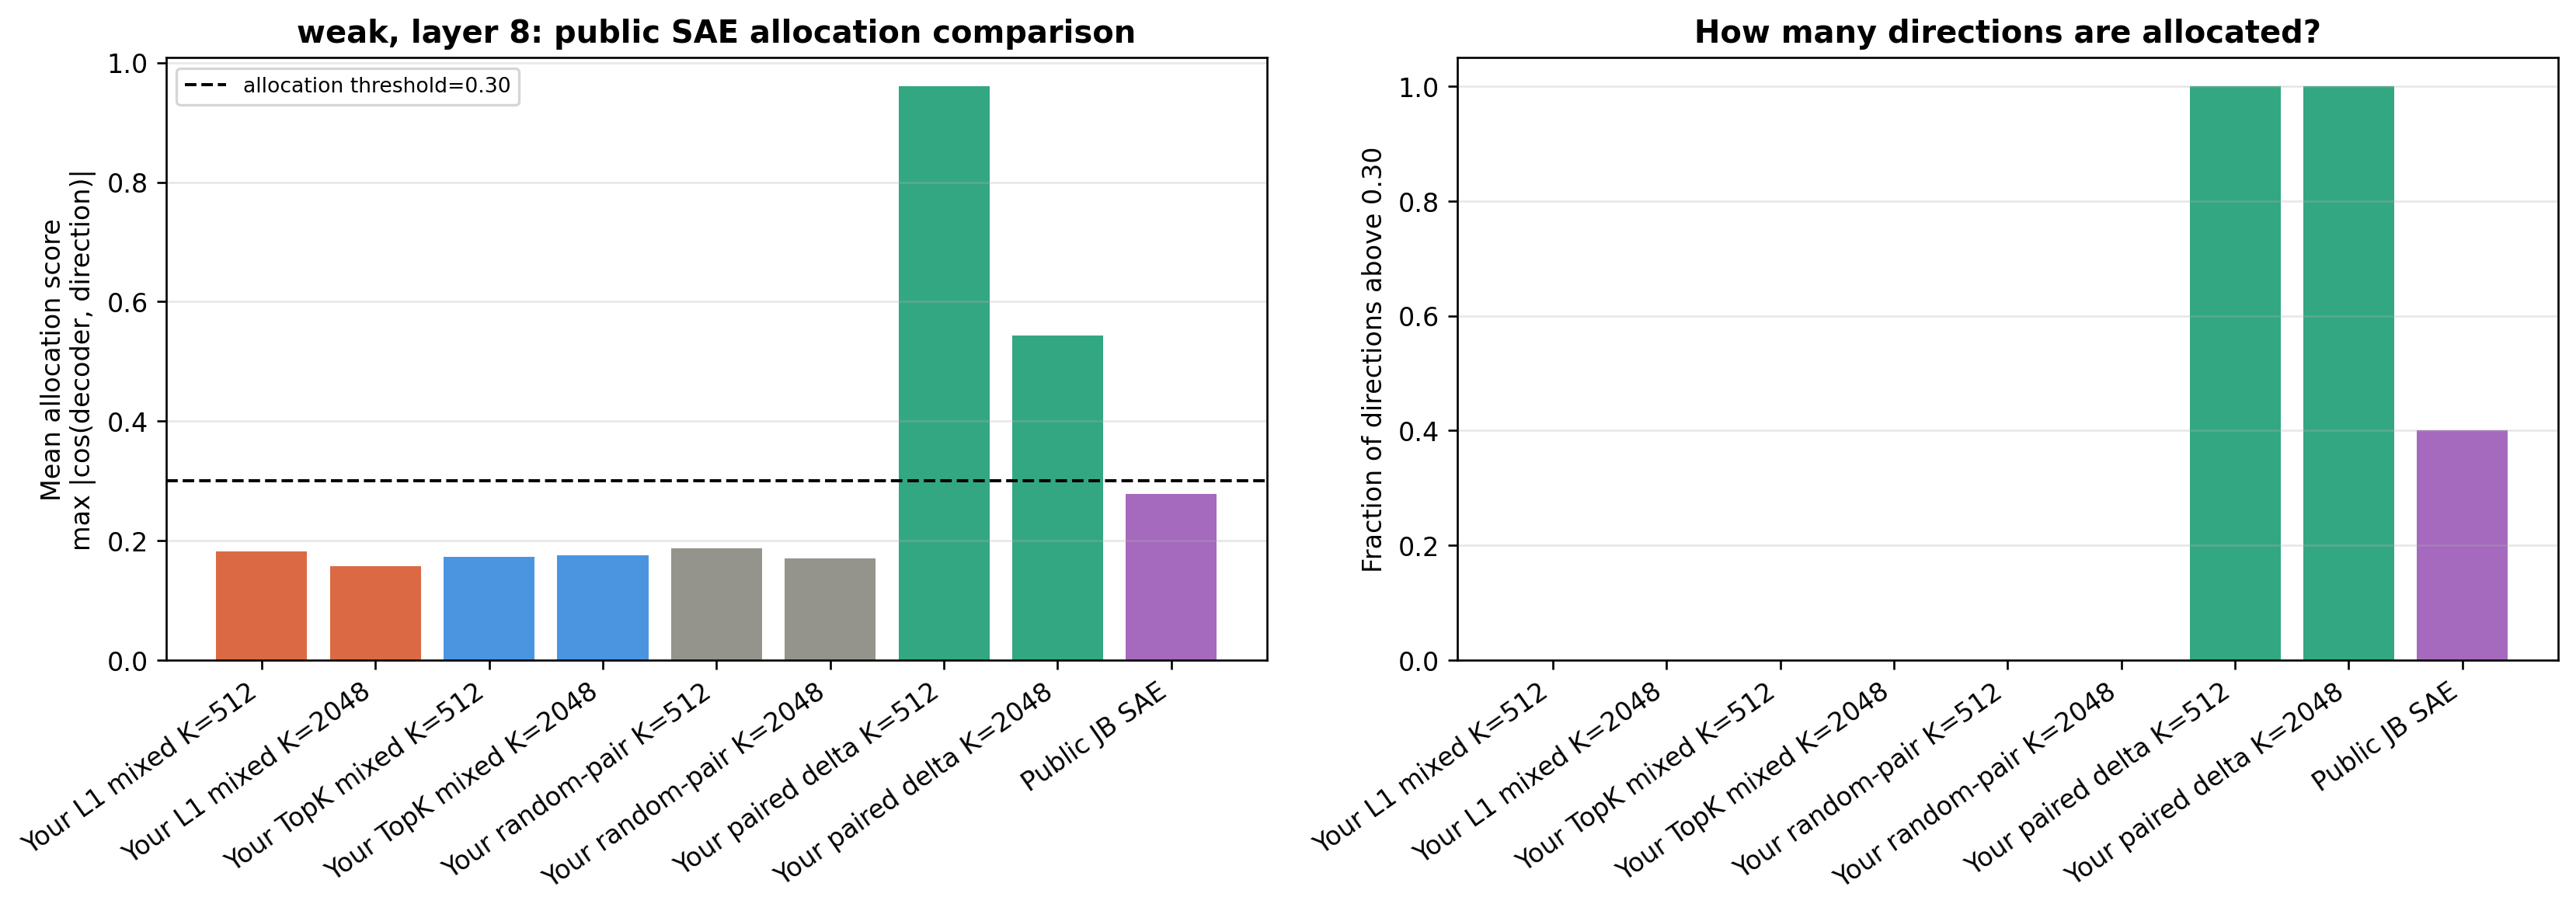
\includegraphics[width=0.75\linewidth]{figures/public_vs_internal_allocation_weak_layer8.png}
\caption{Mean decoder allocation to weak target directions across SAE training conditions, with a publicly released GPT-2-small residual-stream SAE on the right. Mixed/random-pair training and the public SAE cluster at $\sim$0.2--0.3 allocation. Paired-delta reaches $\sim$0.95. The dashed line at 0.30 is a heuristic reference threshold used in this analysis.}
\end{figure}

The claim is not that public SAE features are poor. The claim is that the geometric allocation signal alone, at the level public SAEs produce, does not distinguish ``has actually learned this direction as a selective feature'' from ``has not.'' That distinction requires a functional test on selectivity, recovery, or a downstream causal intervention, not just decoder cosine similarity.

\section*{Next steps}

The result is sharp at GPT-2-small. Natural next experiments, in priority order:

\begin{enumerate}\setlength\itemsep{0em}\setlength{\parskip}{0pt}
  \item \textbf{Does the gap survive at scale?} Replicate at Gemma-2-2B (and headline-only at Gemma-2-9B). Gemma Scope provides high-quality public SAEs at both scales, extending the natural-feature comparison.
  \item \textbf{Does it survive bigger capacity?} K=4096, K=8192. Closes the capacity objection cleanly.
  \item \textbf{Does it survive other SAE recipes?} JumpReLU, gated, batch-TopK.
  \item \textbf{Does it hold for natural features, not just injected ones?} Use Gemma Scope's documented features as the target directions.
  \item \textbf{Toy-model sanity check.} Anthropic's ``Toy Models of Superposition'' setup with known ground-truth features, to verify the recovery metric does what it claims when features genuinely exist.
\end{enumerate}

If the gap survives Gemma-2-2B with larger capacities, multiple SAE recipes, and natural-feature comparisons, the result would become substantially stronger.

\section*{Limitations}

The current artifact is strongest as a controlled diagnostic result on GPT-2-small with injected target directions, not naturally occurring features. Absolute allocation thresholds (e.g.\ the 0.30 line) shouldn't be read as universal as they depend on dimensionality and noise floor. The paired-delta condition is a positive control, not a recommended training recipe; isolating one direction at a time is what makes it succeed, and that's not what reconstruction-SAE practice is trying to do. The claim here is narrow and methodological: at this scale, with these recipes, decoder alignment is not sufficient evidence of functional feature recovery, and the two diagnostics should be reported together.

\end{document}